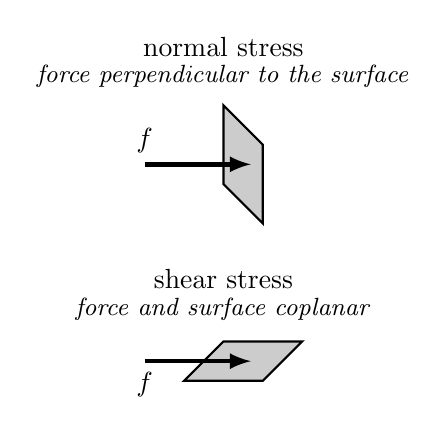
\begin{tikzpicture}
		\begin{scope}[xshift=1cm]
			\draw [fill, color = black, fill opacity=0.2, thick]
			(5cm, 2.5cm) -- (5.5cm, 2cm)
			-- (5.5cm, 1cm) -- (5cm, 1.5cm) -- cycle ;
			\node at (5cm, 3cm) [above] {normal stress};
			\node at (5cm, 2.60cm) [above]
			{\small \textit{force perpendicular to the surface}};

			\draw [-latex, ultra thick] (4cm, 1.75cm) -- (5.35cm, 1.75cm)
			node [above, pos=0] {$\vb{f}$};

			\node at (5cm, 0.05cm) [above] {shear stress};
			\node at (5cm, -0.35cm) [above]
			{\small \textit{force and surface coplanar}};
			\draw [fill, color = black, fill opacity=0.2, thick]
			(5cm, -0.5cm) -- (6cm, -0.5cm) -- (5.5cm, -1cm)
			-- (4.5cm, -1cm) -- cycle;
			\draw [-latex, ultra thick] (4cm, -0.75cm) -- (5.35cm, -0.75cm)
			node [below, pos=0] {$\vb{f}$};
		\end{scope}
\end{tikzpicture}
